\documentclass[a4paper,11pt]{article}
\usepackage{graphicx} % Required for inserting images
\usepackage{amsmath}  % Required for align environment
\usepackage{amssymb}
\usepackage{float}    % Control figure placement
\usepackage{tikz}     % Drawing and diagrams
\usepackage{hyperref}
\usepackage{geometry}
\geometry{margin=1in}

\title{Assignment B3: State estimation}
\author{Jestin, Cormaccar, Conal and Balaji Baskaran}
\date{15th Feburary 2025}

\begin{document}

\maketitle
The Repository link: \href{https://github.com/balajibaski/Vehicle_Estimator/tree/main}{Vehicle Estimator}
\section*{State Space modeling}

\subsection*{State Equation}
% i think we have to change the dynamics, since in theory we are doing in a 2-D plane the dynamics will also change right, so based on the A matrix in therory we have to change the system dynamics as well
The state equation represents the evolution of the system's state \( \mathbf{x}_t \) over time. We assume the system to follow a \textbf{ constant turn rate and velocity (CTRV) },  with state vector $\mathbf{x} = [x, y, v, \theta]^T$, where $\theta$ is the heading angle.
\subsection*{State Transition Equations}
\begin{align*}
    x_{k+1} &= x_k + v_k \cos(\theta_k) \Delta t \\
    y_{k+1} &= y_k + v_k \sin(\theta_k) \Delta t \\
    v_{k+1} &= v_k \quad \text{(constant velocity)} \\
    \theta_{k+1} &= \theta_k + \omega \Delta t \quad \text{(constant angular velocity)}
\end{align*}
Here, $\omega = 1$ rad/s is \textbf{incorrectly assumed} in the code (does not match true $\omega_A$ or $\omega_B$).

\subsection*{Linearized State Transition Matrix ($F$)}
The state transition matrix $F$ is responsible for propagating the state forward in time based on the system's motion model. It is defined as:
\begin{equation*}
    F =
    \begin{bmatrix}
        1 & 0 & \cos(\theta)\Delta t & -v \sin(\theta)\Delta t \\
        0 & 1 & \sin(\theta)\Delta t & v \cos(\theta)\Delta t \\
        0 & 0 & 1 & 0 \\
        0 & 0 & 0 & 1
    \end{bmatrix}
\end{equation*}
where $v$ is the velocity and $dt$ is the time step.
Derived from the Jacobian of the nonlinear motion model.
For this system:
\[
\mathbf{x}_{t+1} = 
\begin{bmatrix}
1 & T_s \\
0 & 1
\end{bmatrix} \begin{bmatrix}
   \mathbf{x}_t \\ \mathbf{v}_{t} 
\end{bmatrix}
 +
\begin{bmatrix}
0 \\
1
\end{bmatrix}
\mathbf{w}_{t}
\]

\subsection*{Process Noise Covariance Matrix ($Q$)}
The process noise covariance matrix $Q$ models the uncertainty in the motion model, accounting for variations in position and orientation:
\begin{equation}
Q = \begin{bmatrix}
\sigma_x^2 & 0 & 0 \\
0 & \sigma_y^2 & 0 \\
0 & 0 & \sigma_\theta^2
\end{bmatrix}
\end{equation}
where $\sigma_x^2$, $\sigma_y^2$, and $\sigma_\theta^2$ represent the variances of position and heading noise, respectively. This matrix helps to balance prediction confidence and measurement updates.

\subsection*{Measurement Model}
\begin{equation*}
    \mathbf{z} = H\mathbf{x} + \mathbf{w}, \quad 
    \end{equation*}

where:
\[
H =
\begin{bmatrix}
\frac{x - b_{x1}}{d_1} & \frac{y - b_{y1}}{d_1} & 0 \\
\frac{x - b_{x2}}{d_2} & \frac{y - b_{y2}}{d_2} & 0 \\
\frac{x - b_{x3}}{d_3} & \frac{y - b_{y3}}{d_3} & 0
\end{bmatrix}
\text{and } d_i = \sqrt{(x - b_{xi})^2 + (y - b_{yi})^2}
\]

\section*{Estimation using Extended Kalman Filter (EKF)}

The EKF is used to estimate the system states given noisy observations. The steps involved are:

\subsection*{Prediction Step}
\begin{itemize}
    \item Compute the predicted state using the nonlinear state transition model:
    \begin{equation}
        \hat{x}_{k|k-1} = f(\hat{x}_{k-1}, u_k)
    \end{equation}
    \item Compute the predicted covariance:
    \begin{equation}
        P_{k|k-1} = F_k P_{k-1} F_k^T + Q_k
    \end{equation}
    where $F_k$ is the Jacobian of $f(x)$ with respect to $x$, and $Q_k$ is the process noise covariance.
\end{itemize}

\subsection*{Measurement Update Step}
\begin{itemize}
    \item Compute the Kalman gain:
    \begin{equation}
        K_k = P_{k|k-1} H_k^T (H_k P_{k|k-1} H_k^T + R_k)^{-1}
    \end{equation}
    where $H_k$ is the Jacobian of the measurement function $h(x)$ with respect to $x$, and $R_k$ is the measurement noise covariance.
    \item Update the state estimate:
    \begin{equation}
        \hat{x}_k = \hat{x}_{k|k-1} + K_k (y_k - h(\hat{x}_{k|k-1}))
    \end{equation}
    \item Update the error covariance:
    \begin{equation}
        P_k = (I - K_k H_k) P_{k|k-1}
    \end{equation}
\end{itemize}


%This model captures the system's dynamics and measurements, suitable for use in state estimation techniques like the Extended Kalman Filter (EKF). This filter uses the following equation to predict and update the system: 
%\subsection*{Prediction Step (Time Update)}
%\begin{align*}
%\hat{x}_{t|t-1} &= f(\hat{x}_{t-1|t-1}, 0) \\
%P_{t|t-1} &= A P_{t-1|t-1} A^T + Q
%\end{align*}
%where: 
%\begin{itemize}
%    \item \( \hat{x}_{t|t-1} \) is Predicted state estimate (before measurement update)
%    \item \( P_{t|t-1} \) is Predicted error covariance matrix
%    \item \( A \) is State transition matrix (Jacobian of \( f(x) \))
%    \item \( Q \) is Process noise covariance
%\end{itemize}
%\subsection*{Update Step (Measurement Update)}
%\begin{align*}
%K_t &= P_{t|t-1} C_t^T (C_t P_{t|t-1} C_t^T + R)^{-1} \\
%\hat{x}_{t|t} &= \hat{x}_{t|t-1} + K_t \left( y_t - h(\hat{x}_{t|t-1}) \right) \\
%P_{t|t} &= P_{t|t-1} - K_t C_t P_{t|t-1}
%\end{align*}
%where:
%\begin{itemize}
%    \item \( K_t \) is Kalman gain
%    \item \( C_t \) is Jacobian of the measurement function \( h(x) \)
%    \item \( R \) is Measurement noise covariance
%    \item \( \hat{x}_{t|t} \) is Updated state estimate after incorporating measurement \( y_t \)
%    \item \( P_{t|t} \) is Updated error covariance
%\end{itemize}
%The state model has been extended for the system represents an object moving in 2D space with:
%\begin{itemize}
%    \item Position \( (x,y) \).
%    \item Velocity \( (v_x,v_y) \).
%\end{itemize}
%The state equations are given as
%\[\mathbf{x}_{t+1} = \mathbf{x}_t + T_s \mathbf{v}_{x}\]
%\[\mathbf{y}_{t+1} = \mathbf{y}_t + T_s \mathbf{v}_{y}\]
%\[v_{\mathbf{x}_{t+1}} = \mathbf{v}_x + \mathbf{w}_{x}\]
%\[v_{\mathbf{y}_{t+1}} = \mathbf{v}_y + \mathbf{w}_{y}\]
%where:
%\begin{itemize}
%    \item \(T_s\) is sampling time.
%    \item \(\mathbf{w}_{x} \text{ and } \mathbf{w}_{y}\) are process noise affecting velocity.
%\end{itemize}
%This state vector \(\begin{bmatrix}
%    \mathbf{x}_t + T_s \mathbf{v}_{x} & \mathbf{y}_t + T_s \mathbf{v}_{y}
%& \mathbf{v}_x + \mathbf{w}_{x}
%& \mathbf{v}_y + \mathbf{w}_{y}
%\end{bmatrix}^T\) effectively captures both position and velocity, which are necessary for predicting future states in a dynamic system. The state transition matrix \(A\) is give as
%\[A = \begin{bmatrix}
%    1 & 0 & T_s & 0 \\ 
%    0 & 1 & 0 & T_s \\
%    0 & 0 & 1 & 0 \\
%    0 & 0 & 0 & 1 \\ \end{bmatrix}\]
%In measurement model, since we do not measure the velocity directly, the function is only depended on the position \((x,y)\). It is given as
%\[
%\mathbf{z}_{t} = h( \mathbf{x}_t,\mathbf{u}_{t})
%\]
%where \(\mathbf{z}_{t} = \begin{bmatrix}
%    d_1 & d_2 & d_3
%\end{bmatrix}^T + \begin{bmatrix}
%    \mathbf{u}_1 & \mathbf{u}_2 & \mathbf{u}_3
%\end{bmatrix}^T\) and \(d_i\) is the Euclidean distance between the vehicle's position to the \(i^{th}\) beacon. As this is a non-linear function we use Jacobian matrix \((\frac{\partial h}{\partial \mathbf{x}})\) to linearize it for the EKF update.
%
%The estimation of the state of a system deals with uncertainties and arises from:
%\begin{itemize}
%    \item Process noise: The uncertainty in the system states and is given by the process noise covariance matrix \((Q)\).
%    \item Measurement noise: The uncertainty in the measurement is states and is given by the measurement noise covariance matrix \((R)\).
%\end{itemize}
%The extended process noise matrix \(Q 
%_{bar}\)is used for the full position-velocity state:
% also I think we can do exactly as how its given in the notes, like giving the equation of  Q_bar and A. Then we can say that since the system is linear, that the Jacobian becomes the A matrix and Q_bar is givrn by the formula Q_bar = GQG^T
%\[Q_{bar} = \begin{bmatrix}
%    0 & 0 & 0 & 0 \\ 0 & 0 & 0 & 0 \\
%0 & 0 & \mathbf{w}_{x} & 0 \\ 0 & 0 & 0 & \mathbf{w}_{y} \\ \end{bmatrix}\]
%The noise is added only in the velocity block and not in the position block because it does not affect the position. 
%
%The matrix \(R\) determines the noise of the sensor's readings and as there are 3 beacons, \(R\) can be represented as \(3 \times 3\) diagonal matrix, which is:
% Check the R matrix once more, it the noise variance of the measurement and i have made it as a identity matrix
%\[R = \begin{bmatrix}
%     \mathbf{u}_1 & 0 & 0 \\ 0 & \mathbf{u}_2 & 0 \\
%0 & 0 & \mathbf{u}_3  \end{bmatrix}\]
%The filter is calculated using python running for 50 iterations which computes measurement prediction and updates the state estimate using the EKF update equations and the next state is predicted using system dynamics. 

\section*{Track Geometry}
The track consists of two arcs of a circle and two linear segments, representing a transition between one motion regime and another.

\subsection*{Track Sections}

\paragraph{First Circular Motion (Radius $r_A = 48$)}
The object moves in a counterclockwise direction along a circular path with a radius of 48 units. The interval of angles covers:
\begin{equation}
\theta = 0 \text{ to } \theta_1.
\end{equation}
The transition occurs at:
\begin{equation}
\theta_1 = 15^\circ,
\end{equation}
where the motion changes from circular to straight-line motion.

\paragraph{First Straight-Line Motion}
After the first circular segment, the object travels in a straight line at constant velocity:
\begin{equation}
v = 10 \text{ units/sec}.
\end{equation}
The endpoint of the linear segment is defined by a transition time preset.

\paragraph{Second Circular Motion (Radius $r_B = 22$)}
The object now traverses a smaller arc in a clockwise fashion with:
\begin{equation}
r_B = 22.
\end{equation}
The object follows an angular displacement up to:
\begin{equation}
\theta_B = 140^\circ.
\end{equation}

\paragraph{Second Straight-Line Motion}
Similar to the first linear segment, the second linear motion proceeds at a constant speed in a straight line. This segment ends at the beginning of the final circular arc.

\paragraph{Final Circular Motion (Radius $r_A = 48$)}
The object returns to a circular motion with the original radius:
\begin{equation}
r_A = 48.
\end{equation}
The angular displacement is:
\begin{equation}
\theta_5 = 250^\circ.
\end{equation}
The track closes back to the starting point.

\subsection*{Transition Points}
The transition points between circular and linear motion are defined by the angles and distances:
\begin{equation}
(x_1, y_1), (x_2, y_2), (x_3, y_3), (x_4, y_4)
\end{equation}
mark the end/start of circular and linear segments. These values were manually measured in the code.

\subsection*{Key Observations}
The circular segments follow the equations of a circle:
\begin{equation}
    x = r \cos(\theta), \quad y = r \sin(\theta).
\end{equation}
The linear segments follow simple kinematic equations:
\begin{equation}
    x = x_0 + v \cos(\theta) \cdot t, \quad y = y_0 + v \sin(\theta) \cdot t.
\end{equation}
The transition between sections is controlled by predefined transition times.

\section*{Time Discretization}
Time discretization is essential for simulating the motion numerically. Instead of treating time as a continuous variable, it is divided into small intervals.

\subsection*{How Discretization is Implemented}
\paragraph{Total Simulation Time}
The total simulation time is set to 43 seconds.

\paragraph{Number of Time Steps}
The motion is discretized into 500 intervals:
More intervals mean higher accuracy, but also more computations.

\paragraph{Time Step}
The time step is calculated as:
\begin{equation}
dt = \frac{\text{total time}}{\text{number of time steps}}
\end{equation}

This ensures that the simulation updates at regular time intervals.

\paragraph{Time Array ($t$)}
A numpy array stores the discrete time points:
This divides the total time into evenly spaced points for simulation.

\subsection*{Importance of time Discretization}
Larger time step ($dt$) can also speed up the computation, which means that the simulation will become more efficient. But this does not improve accuracy; it would lose significant details of the motion with a larger $dt$, causing poor tracking of fast-moving objects and possible instability of the results.

However, one needs to balance the efficiency of computing and the infidelity-induced errors, and such a decision would be application-dependent and require definition of the desired level of precision in tracking the motion with the corresponding choice of $dt$.

\section*{Results and Discussions}

\subsection*{Results}
We were able to create a system dynamics that simulates the motion of the vehicle in the given track.

\begin{figure} [H]
    \centering
    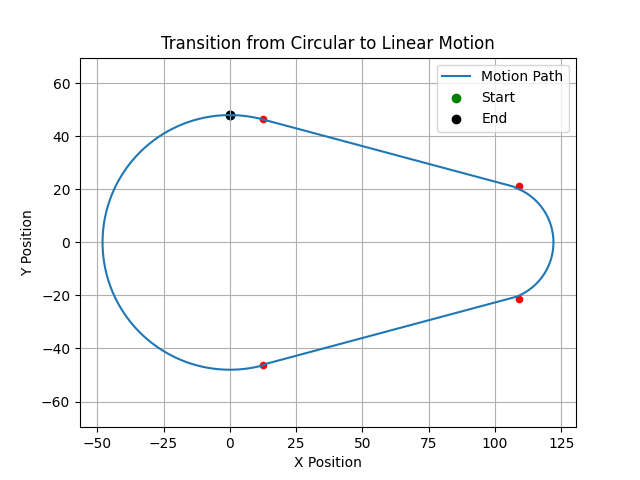
\includegraphics[width=0.8\linewidth]{B3_pics/Figure_1.png}
    \caption{True Dynamics of the vehicle}
    \label{fig:1}
\end{figure}

Using this Dynamics, we tried to estimate the system using Kalamn Filter, considering there are no beacons, and we get the accurate measurements.
\begin{figure} [H]
    \centering
    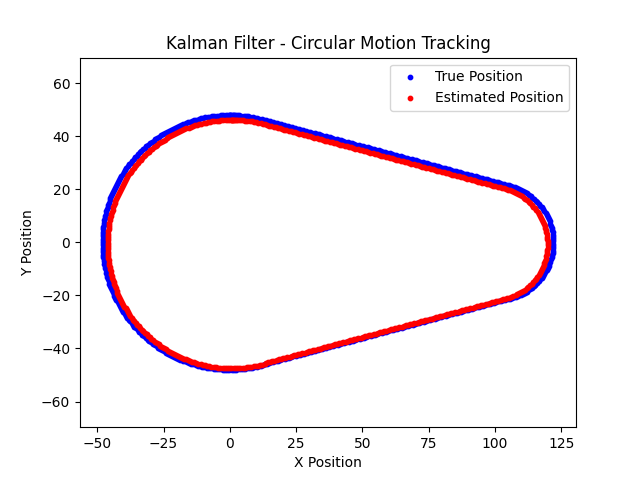
\includegraphics[width=0.8\linewidth]{B3_pics/Figure_2.png}
    \caption{Estimation using Kalaman Filter}
    \label{fig:2}
\end{figure}

 As seen from figure \ref{fig:2} Using the Kalaman Filter, we were able to get good estimator but sinice Kalaman filter couldn't handle the non linear dynamics when the beacon is considered. We went with Extended Kalaman Filter. The below figure shows the estimation from EKF.

\begin{figure} [H]
    \centering
    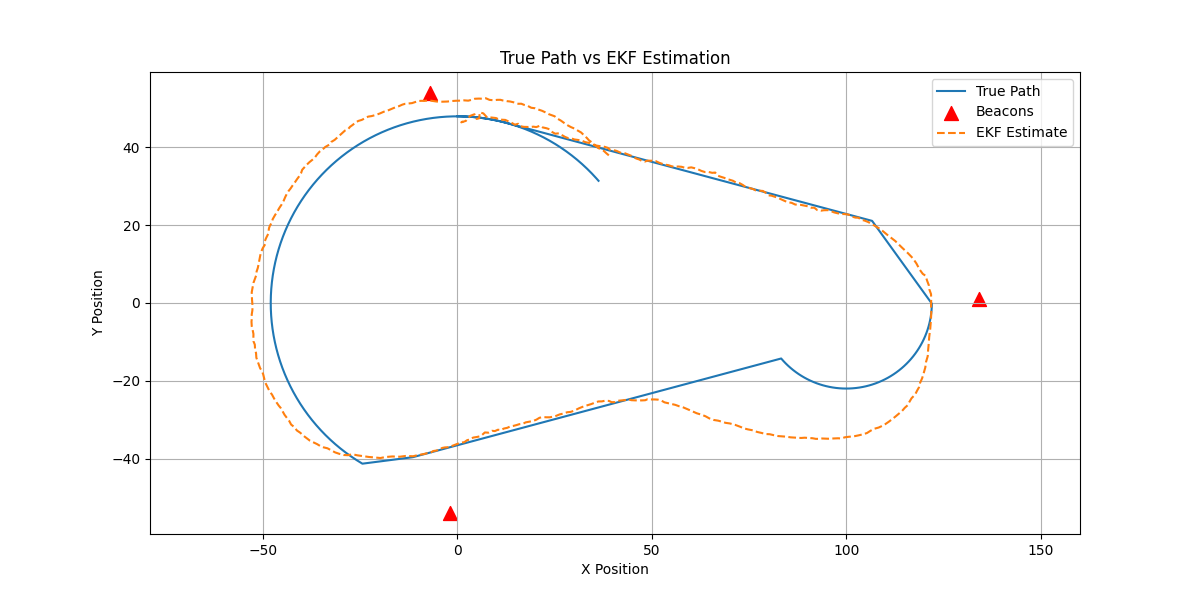
\includegraphics[width=0.8\linewidth]{B3_pics/Figure_3.png}
    \caption{Estimation using Extended Kalaman Filter}
    \label{fig:3}
\end{figure}
As seen from figure \ref{fig:3}, While using the EKF for complex non-linear dynamics, the estimator doesn't do a very good job. We can say the estimation is poor and also EKF cant handle the constraints very well which resulted in this poor estimation.
To handle constraints and non-linear dynamics, one of the estimator to be used is Moving Horizon Estimator. We have done MHE for simpler dynamics and found out that MHE provides really good estimation.

\begin{figure} [H]
    \centering
    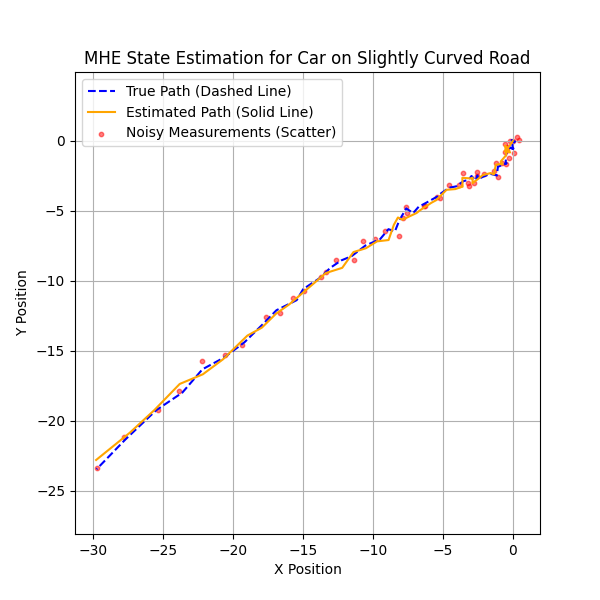
\includegraphics[width=0.8\linewidth]{B3_pics/Figure_4.png}
    \caption{Estimation using Moving Horizon Estimator}
    \label{fig:4}
\end{figure}



\subsection*{Trajectory Plot}
The trajectory plot shows the motion of the object along the track and indicates transitions from circular to linear motion. The visual representation, portrays the overall motion pattern and enables the assessment of numerical simulation accuracy. 
%\begin{figure} [H]
%    \centering
%    \includegraphics[width=0.8\linewidth]{B3_pics/Circular_to_Linear.png}
%    \caption{Timetable of the Project}
%    \label{fig:1}
%\end{figure}
Smoothness of the trajectory depends on time step size and filtering used for state estimation. 

\subsection*{Impact of Noise on the Filter}
In addition to introducing perturbations in location estimations that diverge from the real trajectory, measurement noise also compromises the accuracy of the Kalman filter. The filter may result in unstable estimates and contribute to unpredictable corrections during state updates when the noise level is really high. A properly calibrated Kalman filter reduces noise while maintaining sensitivity to erratic abrupt motion changes.

\subsection*{Approximation Challenges}
One of the primary challenges of motion tracking is that non-linear dynamics must often be approximated by linear estimation models. In this case, the Kalman filter assumes an error distribution that is Gaussian and a linearized model of state transition that does not necessarily correspond to actual dynamics (especially during sharp transitions between circular and linear motion). These approximations will introduce an inconsistency between the performance of simulated and actual trajectories and tracking accuracy. 

\subsection*{Future Enhancement}
To improve accuracy and robustness in state estimation, Moving Horizon Estimator (MHE) can be implemented. A simple dynamics MHE is performed in the script:
\begin{verbatim}
"MHE_simple_dynamics.py"
\end{verbatim}
in the repository and the reason, MHE is more accurate than EKF as that improves estimation by using a window of historical measurements when the measures are available as sets. MHE solves an optimization issue at each iteration, producing a better approximation of non-linear dynamics than the EKF, which updates recursively in local updates. Additionally, EKF is prescriptive for fixed Gaussian noise, which may not function well in most real-world scenarios, whereas MHE fully handles noise fluctuation. Stimulated states and input limitations, which ensure that estimations are physically possible—a luxury that EKF lacks—are another benefit of MHE scanners. 

\end{document}
